\documentclass[twoside]{book}

% Packages required by doxygen
\usepackage{calc}
\usepackage{doxygen}
\usepackage{graphicx}
\usepackage[utf8]{inputenc}
\usepackage{makeidx}
\usepackage{multicol}
\usepackage{multirow}
\usepackage{textcomp}
\usepackage[table]{xcolor}

% Font selection
\usepackage[T1]{fontenc}
\usepackage{mathptmx}
\usepackage[scaled=.90]{helvet}
\usepackage{courier}
\usepackage{amssymb}
\usepackage{sectsty}
\renewcommand{\familydefault}{\sfdefault}
\allsectionsfont{%
  \fontseries{bc}\selectfont%
  \color{darkgray}%
}
\renewcommand{\DoxyLabelFont}{%
  \fontseries{bc}\selectfont%
  \color{darkgray}%
}

% Page & text layout
\usepackage{geometry}
\geometry{%
  a4paper,%
  top=2.5cm,%
  bottom=2.5cm,%
  left=2.5cm,%
  right=2.5cm%
}
\tolerance=750
\hfuzz=15pt
\hbadness=750
\setlength{\emergencystretch}{15pt}
\setlength{\parindent}{0cm}
\setlength{\parskip}{0.2cm}
\makeatletter
\renewcommand{\paragraph}{%
  \@startsection{paragraph}{4}{0ex}{-1.0ex}{1.0ex}{%
    \normalfont\normalsize\bfseries\SS@parafont%
  }%
}
\renewcommand{\subparagraph}{%
  \@startsection{subparagraph}{5}{0ex}{-1.0ex}{1.0ex}{%
    \normalfont\normalsize\bfseries\SS@subparafont%
  }%
}
\makeatother

% Headers & footers
\usepackage{fancyhdr}
\pagestyle{fancyplain}
\fancyhead[LE]{\fancyplain{}{\bfseries\thepage}}
\fancyhead[CE]{\fancyplain{}{}}
\fancyhead[RE]{\fancyplain{}{\bfseries\leftmark}}
\fancyhead[LO]{\fancyplain{}{\bfseries\rightmark}}
\fancyhead[CO]{\fancyplain{}{}}
\fancyhead[RO]{\fancyplain{}{\bfseries\thepage}}
\fancyfoot[LE]{\fancyplain{}{}}
\fancyfoot[CE]{\fancyplain{}{}}
\fancyfoot[RE]{\fancyplain{}{\bfseries\scriptsize Generated on Sat May 5 2018 20\-:11\-:43 for My Project by Doxygen }}
\fancyfoot[LO]{\fancyplain{}{\bfseries\scriptsize Generated on Sat May 5 2018 20\-:11\-:43 for My Project by Doxygen }}
\fancyfoot[CO]{\fancyplain{}{}}
\fancyfoot[RO]{\fancyplain{}{}}
\renewcommand{\footrulewidth}{0.4pt}
\renewcommand{\chaptermark}[1]{%
  \markboth{#1}{}%
}
\renewcommand{\sectionmark}[1]{%
  \markright{\thesection\ #1}%
}

% Indices & bibliography
\usepackage{natbib}
\usepackage[titles]{tocloft}
\setcounter{tocdepth}{3}
\setcounter{secnumdepth}{5}
\makeindex

% Hyperlinks (required, but should be loaded last)
\usepackage{ifpdf}
\ifpdf
  \usepackage[pdftex,pagebackref=true]{hyperref}
\else
  \usepackage[ps2pdf,pagebackref=true]{hyperref}
\fi
\hypersetup{%
  colorlinks=true,%
  linkcolor=blue,%
  citecolor=blue,%
  unicode%
}

% Custom commands
\newcommand{\clearemptydoublepage}{%
  \newpage{\pagestyle{empty}\cleardoublepage}%
}


%===== C O N T E N T S =====

\begin{document}

% Titlepage & ToC
\hypersetup{pageanchor=false}
\pagenumbering{roman}
\begin{titlepage}
\vspace*{7cm}
\begin{center}%
{\Large My Project }\\
\vspace*{1cm}
{\large Generated by Doxygen 1.8.6}\\
\vspace*{0.5cm}
{\small Sat May 5 2018 20:11:43}\\
\end{center}
\end{titlepage}
\clearemptydoublepage
\tableofcontents
\clearemptydoublepage
\pagenumbering{arabic}
\hypersetup{pageanchor=true}

%--- Begin generated contents ---
\chapter{Hierarchical Index}
\section{Class Hierarchy}
This inheritance list is sorted roughly, but not completely, alphabetically\-:\begin{DoxyCompactList}
\item \contentsline{section}{Cache\-Entry}{\pageref{structCacheEntry}}{}
\item \contentsline{section}{Chunk}{\pageref{classChunk}}{}
\item \contentsline{section}{Chunk\-Database}{\pageref{classChunkDatabase}}{}
\item \contentsline{section}{Chunk\-Generator}{\pageref{classChunkGenerator}}{}
\item \contentsline{section}{Chunk\-Tile}{\pageref{structChunkTile}}{}
\item \contentsline{section}{Game}{\pageref{classGame}}{}
\item \contentsline{section}{Object}{\pageref{classObject}}{}
\item \contentsline{section}{State}{\pageref{classState}}{}
\begin{DoxyCompactList}
\item \contentsline{section}{Game\-State}{\pageref{classGameState}}{}
\end{DoxyCompactList}
\item \contentsline{section}{Tile}{\pageref{classTile}}{}
\item \contentsline{section}{Tile\-Database}{\pageref{classTileDatabase}}{}
\item \contentsline{section}{World}{\pageref{classWorld}}{}
\end{DoxyCompactList}

\chapter{Class Index}
\section{Class List}
Here are the classes, structs, unions and interfaces with brief descriptions\-:\begin{DoxyCompactList}
\item\contentsline{section}{\hyperlink{structCacheEntry}{Cache\-Entry} }{\pageref{structCacheEntry}}{}
\item\contentsline{section}{\hyperlink{classChunk}{Chunk} }{\pageref{classChunk}}{}
\item\contentsline{section}{\hyperlink{classChunkDatabase}{Chunk\-Database} }{\pageref{classChunkDatabase}}{}
\item\contentsline{section}{\hyperlink{classChunkGenerator}{Chunk\-Generator} }{\pageref{classChunkGenerator}}{}
\item\contentsline{section}{\hyperlink{classGame}{Game} }{\pageref{classGame}}{}
\item\contentsline{section}{\hyperlink{classGameState}{Game\-State} }{\pageref{classGameState}}{}
\item\contentsline{section}{\hyperlink{classObject}{Object} }{\pageref{classObject}}{}
\item\contentsline{section}{\hyperlink{classState}{State} }{\pageref{classState}}{}
\item\contentsline{section}{\hyperlink{classTile}{Tile} }{\pageref{classTile}}{}
\item\contentsline{section}{\hyperlink{classTileDatabase}{Tile\-Database} }{\pageref{classTileDatabase}}{}
\item\contentsline{section}{\hyperlink{classWorld}{World} }{\pageref{classWorld}}{}
\end{DoxyCompactList}

\chapter{Class Documentation}
\hypertarget{classBiome}{\section{Biome Class Reference}
\label{classBiome}\index{Biome@{Biome}}
}


Collaboration diagram for Biome\-:
\subsection*{Public Member Functions}
\begin{DoxyCompactItemize}
\item 
\hypertarget{classBiome_a407c0e4263eee9af08e90caf1a7b4184}{{\bfseries Biome} (nlohmann\-::json)}\label{classBiome_a407c0e4263eee9af08e90caf1a7b4184}

\end{DoxyCompactItemize}
\subsection*{Public Attributes}
\begin{DoxyCompactItemize}
\item 
\hypertarget{classBiome_a18a3a187676e49e4250a82871bef722f}{int {\bfseries biome\-Id}}\label{classBiome_a18a3a187676e49e4250a82871bef722f}

\item 
\hypertarget{classBiome_a18ad1a11ef83d49b1fbcf925bba29ff5}{\hyperlink{classChunkTile}{Chunk\-Tile} {\bfseries primary\-Tile}}\label{classBiome_a18ad1a11ef83d49b1fbcf925bba29ff5}

\item 
\hypertarget{classBiome_abd58396ce06a2255cf349d08d4ebc4d4}{\hyperlink{classChunkTile}{Chunk\-Tile} {\bfseries surface\-Tile}}\label{classBiome_abd58396ce06a2255cf349d08d4ebc4d4}

\item 
\hypertarget{classBiome_a85cc0f9115bc58dd3d55a8097f832ab8}{\hyperlink{classChunkTile}{Chunk\-Tile} {\bfseries sub\-Surface\-Tile}}\label{classBiome_a85cc0f9115bc58dd3d55a8097f832ab8}

\item 
\hypertarget{classBiome_ac2a44a25fddf50a56602da4553574c52}{std\-::vector$<$ \hyperlink{classSecondaryMaterial}{Secondary\-Material} $>$ {\bfseries secondary\-Materials}}\label{classBiome_ac2a44a25fddf50a56602da4553574c52}

\end{DoxyCompactItemize}
\subsection*{Static Public Attributes}
\begin{DoxyCompactItemize}
\item 
\hypertarget{classBiome_a5358d2284ad8408116e8201c2bf39ac6}{static constexpr auto {\bfseries T\-A\-G} = \char`\"{}Biome\char`\"{}}\label{classBiome_a5358d2284ad8408116e8201c2bf39ac6}

\end{DoxyCompactItemize}


The documentation for this class was generated from the following files\-:\begin{DoxyCompactItemize}
\item 
src/world/chunk/Chunk\-Generator.\-h\item 
src/world/chunk/Chunk\-Generator.\-cpp\end{DoxyCompactItemize}

\hypertarget{structCacheEntry}{\section{Cache\-Entry Struct Reference}
\label{structCacheEntry}\index{Cache\-Entry@{Cache\-Entry}}
}
\subsection*{Public Attributes}
\begin{DoxyCompactItemize}
\item 
\hypertarget{structCacheEntry_aee492f9285bb4a0415414628bd484e5b}{std\-::unique\-\_\-ptr$<$ \hyperlink{classChunk}{Chunk} $>$ {\bfseries chunk}}\label{structCacheEntry_aee492f9285bb4a0415414628bd484e5b}

\item 
\hypertarget{structCacheEntry_a2f38d76a011b952a0d4d3acbbb88b747}{std\-::chrono\-::system\-\_\-clock\-::time\-\_\-point {\bfseries last\-Hit}}\label{structCacheEntry_a2f38d76a011b952a0d4d3acbbb88b747}

\end{DoxyCompactItemize}
\subsection*{Static Public Attributes}
\begin{DoxyCompactItemize}
\item 
\hypertarget{structCacheEntry_ae7717d7b51835ec7486641f72eef5e7e}{static constexpr auto {\bfseries T\-A\-G} = \char`\"{}Cache\-Entry\char`\"{}}\label{structCacheEntry_ae7717d7b51835ec7486641f72eef5e7e}

\end{DoxyCompactItemize}


The documentation for this struct was generated from the following file\-:\begin{DoxyCompactItemize}
\item 
/home/travis/build/\-Z\-S\-A\-Inf\-Project/\-Project\-No\-Name/src/world/chunk/Chunk\-Database.\-h\end{DoxyCompactItemize}

\hypertarget{classChunk}{\section{Chunk Class Reference}
\label{classChunk}\index{Chunk@{Chunk}}
}
\subsection*{Public Member Functions}
\begin{DoxyCompactItemize}
\item 
\hypertarget{classChunk_a698770d828a0a5b98250ce52a8576f4c}{{\bfseries Chunk} (\hyperlink{classChunk}{Chunk} const \&)=delete}\label{classChunk_a698770d828a0a5b98250ce52a8576f4c}

\item 
\hypertarget{classChunk_a739049c7e4b9e6b8d501ff9959e73cee}{void {\bfseries operator=} (\hyperlink{classChunk}{Chunk} const \&)=delete}\label{classChunk_a739049c7e4b9e6b8d501ff9959e73cee}

\item 
\hypertarget{classChunk_a0353e35c14d4f576542660bb762db51f}{void {\bfseries render} (sf\-::\-Render\-Window \&window, const sf\-::\-Vector2f \&translation, const sf\-::\-Vector2f \&scale)}\label{classChunk_a0353e35c14d4f576542660bb762db51f}

\item 
\hypertarget{classChunk_aa794fcda8fe859680cbfe4a2bcd5d097}{void {\bfseries update} (std\-::chrono\-::microseconds delta\-Time)}\label{classChunk_aa794fcda8fe859680cbfe4a2bcd5d097}

\item 
\hypertarget{classChunk_ac3e70286e057eb0f93accec639047097}{void {\bfseries save} (const std\-::string \&filename)}\label{classChunk_ac3e70286e057eb0f93accec639047097}

\item 
\hypertarget{classChunk_afa9fe7d9713cbf4fbe75520dd760880a}{bool {\bfseries load} (const std\-::string \&filename)}\label{classChunk_afa9fe7d9713cbf4fbe75520dd760880a}

\item 
\hypertarget{classChunk_a0e4673d23721ffed257c11499179a4b3}{int {\bfseries get\-Tile} (int x, int y)}\label{classChunk_a0e4673d23721ffed257c11499179a4b3}

\item 
\hypertarget{classChunk_a2027949ed92132d341f4e7c778ce9ebd}{void {\bfseries set\-Tile} (int x, int y, int value)}\label{classChunk_a2027949ed92132d341f4e7c778ce9ebd}

\item 
\hypertarget{classChunk_a140f2fc8f419f8f5f6cf5483abbb365a}{{\bfseries Chunk} (const std\-::array$<$ int, S\-I\-D\-E\-\_\-\-L\-E\-N\-G\-T\-H $\ast$S\-I\-D\-E\-\_\-\-L\-E\-N\-G\-T\-H $>$ \&\-\_\-tiles)}\label{classChunk_a140f2fc8f419f8f5f6cf5483abbb365a}

\end{DoxyCompactItemize}
\subsection*{Static Public Attributes}
\begin{DoxyCompactItemize}
\item 
\hypertarget{classChunk_a219c57f40ca72814048045f066adc46e}{static const int {\bfseries S\-I\-D\-E\-\_\-\-L\-E\-N\-G\-T\-H} = 32}\label{classChunk_a219c57f40ca72814048045f066adc46e}

\item 
\hypertarget{classChunk_a49f5a883393d976a0d8bbc0123e751d1}{static const int {\bfseries T\-I\-L\-E\-\_\-\-S\-I\-Z\-E} = 16}\label{classChunk_a49f5a883393d976a0d8bbc0123e751d1}

\end{DoxyCompactItemize}


The documentation for this class was generated from the following files\-:\begin{DoxyCompactItemize}
\item 
src/world/chunk/Chunk.\-h\item 
src/world/chunk/Chunk.\-cpp\end{DoxyCompactItemize}

\hypertarget{classChunkDatabase}{\section{Chunk\-Database Class Reference}
\label{classChunkDatabase}\index{Chunk\-Database@{Chunk\-Database}}
}


Class that manages \hyperlink{classChunk}{Chunk} storage, loading and generation.  




{\ttfamily \#include $<$Chunk\-Database.\-h$>$}

\subsection*{Public Member Functions}
\begin{DoxyCompactItemize}
\item 
\hyperlink{classChunk}{Chunk} $\ast$ \hyperlink{classChunkDatabase_abcf683d90bbfc79651f0ccc377037c64}{get\-Chunk} (int x, int y)
\begin{DoxyCompactList}\small\item\em Gets \hyperlink{classChunk}{Chunk} from database. \end{DoxyCompactList}\item 
\hyperlink{classChunkDatabase_ac679a24342adcd98d02c3318882651e4}{Chunk\-Database} (std\-::unique\-\_\-ptr$<$ \hyperlink{classChunkGenerator}{Chunk\-Generator} $>$)
\begin{DoxyCompactList}\small\item\em Method for debugging cache. \end{DoxyCompactList}\end{DoxyCompactItemize}
\subsection*{Public Attributes}
\begin{DoxyCompactItemize}
\item 
\hypertarget{classChunkDatabase_ad017d1f92ddf17b747a1ecc88e7343ad}{std\-::map$<$ std\-::tuple$<$ int, int $>$\\*
, \hyperlink{structCacheEntry}{Cache\-Entry} $>$ {\bfseries chunk\-Cache}}\label{classChunkDatabase_ad017d1f92ddf17b747a1ecc88e7343ad}

\end{DoxyCompactItemize}
\subsection*{Static Public Attributes}
\begin{DoxyCompactItemize}
\item 
\hypertarget{classChunkDatabase_adb967e0a364d2e64dea766df6fd00720}{static constexpr auto {\bfseries T\-A\-G} = \char`\"{}Chunk\-Database\char`\"{}}\label{classChunkDatabase_adb967e0a364d2e64dea766df6fd00720}

\end{DoxyCompactItemize}


\subsection{Detailed Description}
Class that manages \hyperlink{classChunk}{Chunk} storage, loading and generation. 

\hyperlink{classChunkDatabase}{Chunk\-Database} stores recently used chunks in cache and loads or generates new chunks if they are not in the cache. 

\subsection{Constructor \& Destructor Documentation}
\hypertarget{classChunkDatabase_ac679a24342adcd98d02c3318882651e4}{\index{Chunk\-Database@{Chunk\-Database}!Chunk\-Database@{Chunk\-Database}}
\index{Chunk\-Database@{Chunk\-Database}!ChunkDatabase@{Chunk\-Database}}
\subsubsection[{Chunk\-Database}]{\setlength{\rightskip}{0pt plus 5cm}Chunk\-Database\-::\-Chunk\-Database (
\begin{DoxyParamCaption}
\item[{std\-::unique\-\_\-ptr$<$ {\bf Chunk\-Generator} $>$}]{\-\_\-chunk\-Generator}
\end{DoxyParamCaption}
)\hspace{0.3cm}{\ttfamily [explicit]}}}\label{classChunkDatabase_ac679a24342adcd98d02c3318882651e4}


Method for debugging cache. 

Returns string representation of cache (what chunks are loaded). 
\begin{DoxyParams}{Parameters}
{\em x} & X coordinate of top-\/left corner \\
\hline
{\em y} & Y coordinate of top-\/right corner \\
\hline
\end{DoxyParams}
\begin{DoxyReturn}{Returns}
string representation of cache 
\end{DoxyReturn}


\subsection{Member Function Documentation}
\hypertarget{classChunkDatabase_abcf683d90bbfc79651f0ccc377037c64}{\index{Chunk\-Database@{Chunk\-Database}!get\-Chunk@{get\-Chunk}}
\index{get\-Chunk@{get\-Chunk}!ChunkDatabase@{Chunk\-Database}}
\subsubsection[{get\-Chunk}]{\setlength{\rightskip}{0pt plus 5cm}{\bf Chunk} $\ast$ Chunk\-Database\-::get\-Chunk (
\begin{DoxyParamCaption}
\item[{int}]{x, }
\item[{int}]{y}
\end{DoxyParamCaption}
)}}\label{classChunkDatabase_abcf683d90bbfc79651f0ccc377037c64}


Gets \hyperlink{classChunk}{Chunk} from database. 

Return a pointer to requested \hyperlink{classChunk}{Chunk}. Any changes to the \hyperlink{classChunk}{Chunk} are going to get saved automatically. 
\begin{DoxyParams}{Parameters}
{\em x} & X coordinate of \hyperlink{classChunk}{Chunk} \\
\hline
{\em y} & Y coordinate of \hyperlink{classChunk}{Chunk} \\
\hline
\end{DoxyParams}
\begin{DoxyReturn}{Returns}
pointer to requested \hyperlink{classChunk}{Chunk} 
\end{DoxyReturn}


The documentation for this class was generated from the following files\-:\begin{DoxyCompactItemize}
\item 
/home/travis/build/\-Z\-S\-A\-Inf\-Project/\-Project\-No\-Name/src/world/chunk/Chunk\-Database.\-h\item 
/home/travis/build/\-Z\-S\-A\-Inf\-Project/\-Project\-No\-Name/src/world/chunk/Chunk\-Database.\-cpp\end{DoxyCompactItemize}

\hypertarget{classChunkGenerator}{\section{Chunk\-Generator Class Reference}
\label{classChunkGenerator}\index{Chunk\-Generator@{Chunk\-Generator}}
}


\hyperlink{classChunk}{Chunk} generator class.  




{\ttfamily \#include $<$Chunk\-Generator.\-h$>$}

\subsection*{Public Member Functions}
\begin{DoxyCompactItemize}
\item 
std\-::unique\-\_\-ptr$<$ \hyperlink{classChunk}{Chunk} $>$ \hyperlink{classChunkGenerator_acb1e4d2b1d2d620a92fd3e311ddd42cf}{generate\-Chunk} (int x, int y)
\begin{DoxyCompactList}\small\item\em Method used to generate new chunks. \end{DoxyCompactList}\item 
\hypertarget{classChunkGenerator_a9e3abe238109f9d8b98fd1eb92d400f8}{void \hyperlink{classChunkGenerator_a9e3abe238109f9d8b98fd1eb92d400f8}{load\-Biomes} (std\-::string filename)}\label{classChunkGenerator_a9e3abe238109f9d8b98fd1eb92d400f8}

\begin{DoxyCompactList}\small\item\em Loads biomes from file using supplied file name. \end{DoxyCompactList}\item 
\hypertarget{classChunkGenerator_a5809da31d94501123d717e4c0367f80a}{{\bfseries Chunk\-Generator} (int seed)}\label{classChunkGenerator_a5809da31d94501123d717e4c0367f80a}

\end{DoxyCompactItemize}
\subsection*{Static Public Attributes}
\begin{DoxyCompactItemize}
\item 
\hypertarget{classChunkGenerator_a007ea7da3f3c609869024be0ea0fc3dd}{static constexpr auto {\bfseries T\-A\-G} = \char`\"{}Chunk\-Generator\char`\"{}}\label{classChunkGenerator_a007ea7da3f3c609869024be0ea0fc3dd}

\end{DoxyCompactItemize}


\subsection{Detailed Description}
\hyperlink{classChunk}{Chunk} generator class. 

This class generates new chunks based on chunk's position and world seed. 

\subsection{Member Function Documentation}
\hypertarget{classChunkGenerator_acb1e4d2b1d2d620a92fd3e311ddd42cf}{\index{Chunk\-Generator@{Chunk\-Generator}!generate\-Chunk@{generate\-Chunk}}
\index{generate\-Chunk@{generate\-Chunk}!ChunkGenerator@{Chunk\-Generator}}
\subsubsection[{generate\-Chunk}]{\setlength{\rightskip}{0pt plus 5cm}std\-::unique\-\_\-ptr$<$ {\bf Chunk} $>$ Chunk\-Generator\-::generate\-Chunk (
\begin{DoxyParamCaption}
\item[{int}]{x, }
\item[{int}]{y}
\end{DoxyParamCaption}
)}}\label{classChunkGenerator_acb1e4d2b1d2d620a92fd3e311ddd42cf}


Method used to generate new chunks. 

\hyperlink{classChunkGenerator_acb1e4d2b1d2d620a92fd3e311ddd42cf}{generate\-Chunk()} is used to procedurally generate new chunks based on it's world cords and seed 
\begin{DoxyParams}{Parameters}
{\em x} & X coordinate of new chunk \\
\hline
{\em y} & Y coordinate of new chunk \\
\hline
\end{DoxyParams}
\begin{DoxyReturn}{Returns}
a newly created chunk 
\end{DoxyReturn}


The documentation for this class was generated from the following files\-:\begin{DoxyCompactItemize}
\item 
/home/travis/build/\-Z\-S\-A\-Inf\-Project/\-Project\-No\-Name/src/world/chunk/Chunk\-Generator.\-h\item 
/home/travis/build/\-Z\-S\-A\-Inf\-Project/\-Project\-No\-Name/src/world/chunk/Chunk\-Generator.\-cpp\end{DoxyCompactItemize}

\hypertarget{classChunkTile}{\section{Chunk\-Tile Class Reference}
\label{classChunkTile}\index{Chunk\-Tile@{Chunk\-Tile}}
}


Representation of a tile in a chunk.  




{\ttfamily \#include $<$Chunk.\-h$>$}

\subsection*{Public Member Functions}
\begin{DoxyCompactItemize}
\item 
\hypertarget{classChunkTile_a9384499af7d00c6822b7f59d356bd6a3}{{\bfseries Chunk\-Tile} (short \hyperlink{classChunkTile_ac7277fa1d196411449a646d3eed73b39}{tile\-Id}, uint \hyperlink{classChunkTile_a29ac3a16c7075941a5c483f1a3372364}{amount})}\label{classChunkTile_a9384499af7d00c6822b7f59d356bd6a3}

\item 
\hypertarget{classChunkTile_a00633aab2a6285d570f880e4cb216831}{{\bfseries Chunk\-Tile} (nlohmann\-::json)}\label{classChunkTile_a00633aab2a6285d570f880e4cb216831}

\end{DoxyCompactItemize}
\subsection*{Public Attributes}
\begin{DoxyCompactItemize}
\item 
\hypertarget{classChunkTile_ac7277fa1d196411449a646d3eed73b39}{short \hyperlink{classChunkTile_ac7277fa1d196411449a646d3eed73b39}{tile\-Id}}\label{classChunkTile_ac7277fa1d196411449a646d3eed73b39}

\begin{DoxyCompactList}\small\item\em \hyperlink{classTile}{Tile} id pointing to data in \hyperlink{classTileDatabase}{Tile\-Database}. \end{DoxyCompactList}\item 
\hypertarget{classChunkTile_a29ac3a16c7075941a5c483f1a3372364}{uint \hyperlink{classChunkTile_a29ac3a16c7075941a5c483f1a3372364}{amount}}\label{classChunkTile_a29ac3a16c7075941a5c483f1a3372364}

\begin{DoxyCompactList}\small\item\em Amount of material in one tile. \end{DoxyCompactList}\end{DoxyCompactItemize}
\subsection*{Static Public Attributes}
\begin{DoxyCompactItemize}
\item 
\hypertarget{classChunkTile_a321f107b80df537c1d2abbe36bf13df1}{static constexpr auto {\bfseries T\-A\-G} = \char`\"{}Chunk\-Tile\char`\"{}}\label{classChunkTile_a321f107b80df537c1d2abbe36bf13df1}

\end{DoxyCompactItemize}


\subsection{Detailed Description}
Representation of a tile in a chunk. 

The documentation for this class was generated from the following files\-:\begin{DoxyCompactItemize}
\item 
src/world/chunk/Chunk.\-h\item 
src/world/chunk/Chunk.\-cpp\end{DoxyCompactItemize}

\hypertarget{classEntity}{\section{Entity Class Reference}
\label{classEntity}\index{Entity@{Entity}}
}


In game moving entity.  




{\ttfamily \#include $<$Entity.\-h$>$}

\subsection*{Public Member Functions}
\begin{DoxyCompactItemize}
\item 
\hypertarget{classEntity_afb2d2dd5bbd30e71802726cd45d630ae}{{\footnotesize template$<$typename T $>$ }\\void {\bfseries add\-Component} (std\-::unique\-\_\-ptr$<$ \hyperlink{classComponent}{Component} $>$ component)}\label{classEntity_afb2d2dd5bbd30e71802726cd45d630ae}

\item 
\hypertarget{classEntity_a369c207eab2aed48053346a58b4cdbe2}{{\footnotesize template$<$typename T $>$ }\\T $\ast$ {\bfseries get\-Component} ()}\label{classEntity_a369c207eab2aed48053346a58b4cdbe2}

\item 
\hypertarget{classEntity_ad42e3c93df543d22f2bbc8f301fe90d7}{{\bfseries Entity} (\hyperlink{classEntity}{Entity} \&old)}\label{classEntity_ad42e3c93df543d22f2bbc8f301fe90d7}

\item 
\hypertarget{classEntity_a897eef416e1bdc1ab34349caac9da97f}{{\bfseries Entity} (nlohmann\-::json json)}\label{classEntity_a897eef416e1bdc1ab34349caac9da97f}

\end{DoxyCompactItemize}
\subsection*{Public Attributes}
\begin{DoxyCompactItemize}
\item 
\hypertarget{classEntity_ab706f432d78dd17aebad2a6b0fadefac}{std\-::unordered\-\_\-map$<$ uint, \\*
std\-::unique\-\_\-ptr$<$ \hyperlink{classComponent}{Component} $>$ $>$ {\bfseries components}}\label{classEntity_ab706f432d78dd17aebad2a6b0fadefac}

\item 
\hypertarget{classEntity_a931b21fbdebb1a5963b4bcab5df128f5}{std\-::string {\bfseries name}}\label{classEntity_a931b21fbdebb1a5963b4bcab5df128f5}

\end{DoxyCompactItemize}
\subsection*{Static Public Attributes}
\begin{DoxyCompactItemize}
\item 
\hypertarget{classEntity_a71274935a057ccb8119a625d1bff7ac4}{static constexpr auto {\bfseries T\-A\-G} = \char`\"{}Entity\char`\"{}}\label{classEntity_a71274935a057ccb8119a625d1bff7ac4}

\end{DoxyCompactItemize}


\subsection{Detailed Description}
In game moving entity. 

Represents entity -\/ object in game that can move. It's position is not quantized. 

The documentation for this class was generated from the following files\-:\begin{DoxyCompactItemize}
\item 
src/entity/Entity.\-h\item 
src/entity/Entity.\-cpp\end{DoxyCompactItemize}

\hypertarget{classGame}{\section{Game Class Reference}
\label{classGame}\index{Game@{Game}}
}


Main program class.  




{\ttfamily \#include $<$Game.\-h$>$}

\subsection*{Public Member Functions}
\begin{DoxyCompactItemize}
\item 
\hypertarget{classGame_ade1d35f91a6fe6b6da70d7caebd174f6}{void \hyperlink{classGame_ade1d35f91a6fe6b6da70d7caebd174f6}{push\-State} (std\-::shared\-\_\-ptr$<$ \hyperlink{classState}{State} $>$ state)}\label{classGame_ade1d35f91a6fe6b6da70d7caebd174f6}

\begin{DoxyCompactList}\small\item\em Push state on stack. \end{DoxyCompactList}\item 
\hypertarget{classGame_a4b33dd67adef59bebadba8a234282c88}{void \hyperlink{classGame_a4b33dd67adef59bebadba8a234282c88}{pop\-State} ()}\label{classGame_a4b33dd67adef59bebadba8a234282c88}

\begin{DoxyCompactList}\small\item\em Pop state from stack. \end{DoxyCompactList}\item 
\hypertarget{classGame_a1ab78f5ed0d5ea879157357cf2fb2afa}{void \hyperlink{classGame_a1ab78f5ed0d5ea879157357cf2fb2afa}{run} ()}\label{classGame_a1ab78f5ed0d5ea879157357cf2fb2afa}

\begin{DoxyCompactList}\small\item\em Start main loop. \end{DoxyCompactList}\item 
\hypertarget{classGame_a586a831ed5ff1283fcf1b96f4eff065c}{{\bfseries Game} (\hyperlink{classGame}{Game} const \&)=delete}\label{classGame_a586a831ed5ff1283fcf1b96f4eff065c}

\item 
\hypertarget{classGame_aa4c0eacd8656e54ec4e94877c453e531}{void {\bfseries operator=} (\hyperlink{classGame}{Game} const \&)=delete}\label{classGame_aa4c0eacd8656e54ec4e94877c453e531}

\end{DoxyCompactItemize}
\subsection*{Static Public Member Functions}
\begin{DoxyCompactItemize}
\item 
\hypertarget{classGame_aa742f626e4b8a5dac8677ef40263716c}{static \hyperlink{classState}{State} \& \hyperlink{classGame_aa742f626e4b8a5dac8677ef40263716c}{get\-State} ()}\label{classGame_aa742f626e4b8a5dac8677ef40263716c}

\begin{DoxyCompactList}\small\item\em Get reference to state on top of the stack. \end{DoxyCompactList}\item 
\hypertarget{classGame_ada9faa2a1f4e1453420adead02fd9865}{static sf\-::\-Render\-Window \& \hyperlink{classGame_ada9faa2a1f4e1453420adead02fd9865}{get\-Render\-Window} ()}\label{classGame_ada9faa2a1f4e1453420adead02fd9865}

\begin{DoxyCompactList}\small\item\em Returns a reference to main render window. \end{DoxyCompactList}\item 
\hypertarget{classGame_ac69a0c5e25c7acb811f4a7b86a2ceb74}{static \hyperlink{classGame}{Game} \& \hyperlink{classGame_ac69a0c5e25c7acb811f4a7b86a2ceb74}{get} ()}\label{classGame_ac69a0c5e25c7acb811f4a7b86a2ceb74}

\begin{DoxyCompactList}\small\item\em Returns reference to singleton object. \end{DoxyCompactList}\end{DoxyCompactItemize}
\subsection*{Public Attributes}
\begin{DoxyCompactItemize}
\item 
std\-::chrono\-::microseconds \hyperlink{classGame_af9f24863bbe8102d1bf5d97aaa449d14}{minimum\-Loop\-Time} = std\-::chrono\-::microseconds(120)
\begin{DoxyCompactList}\small\item\em Minimum time for main loop iteration. \end{DoxyCompactList}\item 
std\-::chrono\-::microseconds \hyperlink{classGame_a65800b8c8afee406d719b404a4a78877}{tick\-\_\-period} = std\-::chrono\-::microseconds(1000000)
\begin{DoxyCompactList}\small\item\em Period between consecutive tick() calls. \end{DoxyCompactList}\end{DoxyCompactItemize}
\subsection*{Static Public Attributes}
\begin{DoxyCompactItemize}
\item 
\hypertarget{classGame_a43d300e0d66811f7317d88e3476d6de3}{static constexpr auto {\bfseries T\-A\-G} = \char`\"{}Game\-Singleton\char`\"{}}\label{classGame_a43d300e0d66811f7317d88e3476d6de3}

\end{DoxyCompactItemize}


\subsection{Detailed Description}
Main program class. 

This class is a singleton. Contains main game loop. Stores all states on stack and calls update(), render() and tick() on top state. Call rate for each can be setup separately. 

\subsection{Member Data Documentation}
\hypertarget{classGame_af9f24863bbe8102d1bf5d97aaa449d14}{\index{Game@{Game}!minimum\-Loop\-Time@{minimum\-Loop\-Time}}
\index{minimum\-Loop\-Time@{minimum\-Loop\-Time}!Game@{Game}}
\subsubsection[{minimum\-Loop\-Time}]{\setlength{\rightskip}{0pt plus 5cm}std\-::chrono\-::microseconds Game\-::minimum\-Loop\-Time = std\-::chrono\-::microseconds(120)}}\label{classGame_af9f24863bbe8102d1bf5d97aaa449d14}


Minimum time for main loop iteration. 

If main loop runs faster than the set up limit it will be slowed down to save C\-P\-U usage. \hypertarget{classGame_a65800b8c8afee406d719b404a4a78877}{\index{Game@{Game}!tick\-\_\-period@{tick\-\_\-period}}
\index{tick\-\_\-period@{tick\-\_\-period}!Game@{Game}}
\subsubsection[{tick\-\_\-period}]{\setlength{\rightskip}{0pt plus 5cm}std\-::chrono\-::microseconds Game\-::tick\-\_\-period = std\-::chrono\-::microseconds(1000000)}}\label{classGame_a65800b8c8afee406d719b404a4a78877}


Period between consecutive tick() calls. 

tick() will be called periodically with a given period 

The documentation for this class was generated from the following files\-:\begin{DoxyCompactItemize}
\item 
src/Game.\-h\item 
src/Game.\-cpp\end{DoxyCompactItemize}

\hypertarget{classGameState}{\section{Game\-State Class Reference}
\label{classGameState}\index{Game\-State@{Game\-State}}
}


\hyperlink{classState}{State} when actual gameplay is present.  




{\ttfamily \#include $<$Game\-State.\-h$>$}



Inheritance diagram for Game\-State\-:
\nopagebreak
\begin{figure}[H]
\begin{center}
\leavevmode
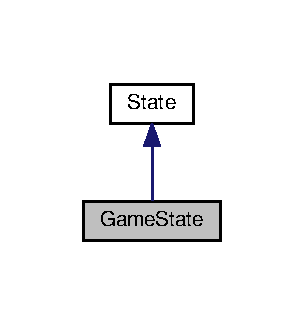
\includegraphics[width=146pt]{classGameState__inherit__graph}
\end{center}
\end{figure}


Collaboration diagram for Game\-State\-:
\nopagebreak
\begin{figure}[H]
\begin{center}
\leavevmode
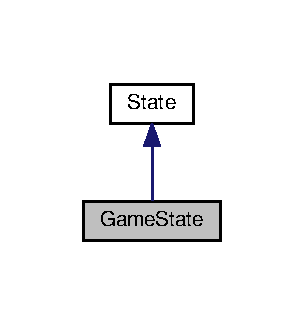
\includegraphics[width=146pt]{classGameState__coll__graph}
\end{center}
\end{figure}
\subsection*{Public Member Functions}
\begin{DoxyCompactItemize}
\item 
void \hyperlink{classGameState_aba059d7ab1a53b8f5d795292ed37abac}{update} (std\-::chrono\-::microseconds delta\-Time) override
\begin{DoxyCompactList}\small\item\em Function called every loop iteration. \end{DoxyCompactList}\item 
void \hyperlink{classGameState_aa4061260f4ca0acc7d1833dbb6691f0f}{render} (float delta\-Time) override
\begin{DoxyCompactList}\small\item\em Function called every screen refresh. \end{DoxyCompactList}\item 
void \hyperlink{classGameState_ae9ff24d75f36ef56daa6a180d4b38a09}{tick} () override
\begin{DoxyCompactList}\small\item\em Function called periodicaly. \end{DoxyCompactList}\item 
\hypertarget{classGameState_a945e9dfe15e3708799977ed8133f7678}{sf\-::\-Vector2f \hyperlink{classGameState_a945e9dfe15e3708799977ed8133f7678}{screen\-\_\-to\-\_\-global\-\_\-offset} (sf\-::\-Vector2f in)}\label{classGameState_a945e9dfe15e3708799977ed8133f7678}

\begin{DoxyCompactList}\small\item\em Converts screen to world coordinates. \end{DoxyCompactList}\item 
\hyperlink{classGameState_a4fa0a2bf50315c4a35a3890a0adcee5c}{Game\-State} ()
\item 
\hypertarget{classGameState_aebc076f9bcec0aa4317eff9e9a8d566e}{\hyperlink{classWorld}{World} \& {\bfseries get\-World} ()}\label{classGameState_aebc076f9bcec0aa4317eff9e9a8d566e}

\item 
\hypertarget{classGameState_a45607b8a0473073090740500826268c0}{sf\-::\-View \& {\bfseries get\-Camera} ()}\label{classGameState_a45607b8a0473073090740500826268c0}

\item 
std\-::shared\-\_\-ptr$<$ \hyperlink{classGameMode}{Game\-Mode} $>$ \hyperlink{classGameState_a20ec39ca6754c9a78e5142772208b1a6}{get\-Game\-Mode} ()
\item 
void \hyperlink{classGameState_a52d8b4a7e3f778f0858ff53554c89eda}{set\-Game\-Mode} (int new\-Mode)
\item 
\hypertarget{classGameState_a64c8327f5ca1d060867381ecfbfd81c3}{std\-::shared\-\_\-ptr$<$ \hyperlink{classGUI}{G\-U\-I} $>$ \hyperlink{classGameState_a64c8327f5ca1d060867381ecfbfd81c3}{get\-G\-U\-I} ()}\label{classGameState_a64c8327f5ca1d060867381ecfbfd81c3}

\begin{DoxyCompactList}\small\item\em Returns a pointer to a \hyperlink{classGUI}{G\-U\-I} object. \end{DoxyCompactList}\end{DoxyCompactItemize}


\subsection{Detailed Description}
\hyperlink{classState}{State} when actual gameplay is present. 

Contains \hyperlink{classWorld}{World}, Entities etc. Get's player input. Runs physics. 

\subsection{Constructor \& Destructor Documentation}
\hypertarget{classGameState_a4fa0a2bf50315c4a35a3890a0adcee5c}{\index{Game\-State@{Game\-State}!Game\-State@{Game\-State}}
\index{Game\-State@{Game\-State}!GameState@{Game\-State}}
\subsubsection[{Game\-State}]{\setlength{\rightskip}{0pt plus 5cm}Game\-State\-::\-Game\-State (
\begin{DoxyParamCaption}
{}
\end{DoxyParamCaption}
)}}\label{classGameState_a4fa0a2bf50315c4a35a3890a0adcee5c}
the same arrangement as in Game\-Mode\-::game\-Modes\-Enum 

\subsection{Member Function Documentation}
\hypertarget{classGameState_a20ec39ca6754c9a78e5142772208b1a6}{\index{Game\-State@{Game\-State}!get\-Game\-Mode@{get\-Game\-Mode}}
\index{get\-Game\-Mode@{get\-Game\-Mode}!GameState@{Game\-State}}
\subsubsection[{get\-Game\-Mode}]{\setlength{\rightskip}{0pt plus 5cm}std\-::shared\-\_\-ptr$<$ {\bf Game\-Mode} $>$ Game\-State\-::get\-Game\-Mode (
\begin{DoxyParamCaption}
{}
\end{DoxyParamCaption}
)}}\label{classGameState_a20ec39ca6754c9a78e5142772208b1a6}
Returns pointer to the active game mode \hypertarget{classGameState_aa4061260f4ca0acc7d1833dbb6691f0f}{\index{Game\-State@{Game\-State}!render@{render}}
\index{render@{render}!GameState@{Game\-State}}
\subsubsection[{render}]{\setlength{\rightskip}{0pt plus 5cm}void Game\-State\-::render (
\begin{DoxyParamCaption}
\item[{float}]{delta\-Time}
\end{DoxyParamCaption}
)\hspace{0.3cm}{\ttfamily [override]}, {\ttfamily [virtual]}}}\label{classGameState_aa4061260f4ca0acc7d1833dbb6691f0f}


Function called every screen refresh. 

\hyperlink{classGameState_aa4061260f4ca0acc7d1833dbb6691f0f}{render()} is called every screen refresh. Should be used for rendering. 
\begin{DoxyParams}{Parameters}
{\em render\-Window} & S\-F\-M\-L render window reference \\
\hline
\end{DoxyParams}


Implements \hyperlink{classState_af989800e12898aea96188086e9fd649d}{State}.

\hypertarget{classGameState_a52d8b4a7e3f778f0858ff53554c89eda}{\index{Game\-State@{Game\-State}!set\-Game\-Mode@{set\-Game\-Mode}}
\index{set\-Game\-Mode@{set\-Game\-Mode}!GameState@{Game\-State}}
\subsubsection[{set\-Game\-Mode}]{\setlength{\rightskip}{0pt plus 5cm}void Game\-State\-::set\-Game\-Mode (
\begin{DoxyParamCaption}
\item[{int}]{new\-Mode}
\end{DoxyParamCaption}
)}}\label{classGameState_a52d8b4a7e3f778f0858ff53554c89eda}
Changes game mode, for list of game modes see \hyperlink{classGameMode}{Game\-Mode} 
\begin{DoxyParams}{Parameters}
{\em new\-Mode} & Get new\-Mode value from Game\-Mode\-::game\-Modes\-Enum \\
\hline
\end{DoxyParams}
\hypertarget{classGameState_ae9ff24d75f36ef56daa6a180d4b38a09}{\index{Game\-State@{Game\-State}!tick@{tick}}
\index{tick@{tick}!GameState@{Game\-State}}
\subsubsection[{tick}]{\setlength{\rightskip}{0pt plus 5cm}void Game\-State\-::tick (
\begin{DoxyParamCaption}
{}
\end{DoxyParamCaption}
)\hspace{0.3cm}{\ttfamily [override]}, {\ttfamily [virtual]}}}\label{classGameState_ae9ff24d75f36ef56daa6a180d4b38a09}


Function called periodicaly. 

\hyperlink{classGameState_ae9ff24d75f36ef56daa6a180d4b38a09}{tick()} is called periodicaly. Period is set in \hyperlink{classGame}{Game} singleton. Can be used for stuff that doesn't need to run very often, for example recalculating A\-I path. 

Implements \hyperlink{classState_a1cdec36e9ffad91ba7af560770601017}{State}.

\hypertarget{classGameState_aba059d7ab1a53b8f5d795292ed37abac}{\index{Game\-State@{Game\-State}!update@{update}}
\index{update@{update}!GameState@{Game\-State}}
\subsubsection[{update}]{\setlength{\rightskip}{0pt plus 5cm}void Game\-State\-::update (
\begin{DoxyParamCaption}
\item[{std\-::chrono\-::microseconds}]{delta\-Time}
\end{DoxyParamCaption}
)\hspace{0.3cm}{\ttfamily [override]}, {\ttfamily [virtual]}}}\label{classGameState_aba059d7ab1a53b8f5d795292ed37abac}


Function called every loop iteration. 

\hyperlink{classGameState_aba059d7ab1a53b8f5d795292ed37abac}{update()} is called every main loop iteration. Should be used for implementing stuff like physics etc. 
\begin{DoxyParams}{Parameters}
{\em delta\-Time} & Time which passed between \hyperlink{classGameState_aba059d7ab1a53b8f5d795292ed37abac}{update()} calls \\
\hline
\end{DoxyParams}


Implements \hyperlink{classState_af2121f8eb52144b7a789214f15e3601a}{State}.



The documentation for this class was generated from the following files\-:\begin{DoxyCompactItemize}
\item 
/home/travis/build/\-Z\-S\-A\-Inf\-Project/\-Project\-No\-Name/src/state/Game\-State.\-h\item 
/home/travis/build/\-Z\-S\-A\-Inf\-Project/\-Project\-No\-Name/src/state/Game\-State.\-cpp\end{DoxyCompactItemize}

\hypertarget{classObject}{\section{Object Class Reference}
\label{classObject}\index{Object@{Object}}
}
\subsection*{Public Member Functions}
\begin{DoxyCompactItemize}
\item 
\hypertarget{classObject_a278a137fafd103884d923fd88c2845cc}{void {\bfseries render} (sf\-::\-Render\-Window)}\label{classObject_a278a137fafd103884d923fd88c2845cc}

\item 
\hypertarget{classObject_ac793c5c56ed16f0309f9eecf2e8e4413}{void {\bfseries click\-On} ()}\label{classObject_ac793c5c56ed16f0309f9eecf2e8e4413}

\item 
\hypertarget{classObject_a81f5c9c6f7806e6b1e13843f0848fdc6}{void {\bfseries update} (std\-::chrono\-::microseconds delta\-Time)}\label{classObject_a81f5c9c6f7806e6b1e13843f0848fdc6}

\end{DoxyCompactItemize}


The documentation for this class was generated from the following files\-:\begin{DoxyCompactItemize}
\item 
/home/travis/build/\-Z\-S\-A\-Inf\-Project/\-Project\-No\-Name/src/world/object/Object.\-h\item 
/home/travis/build/\-Z\-S\-A\-Inf\-Project/\-Project\-No\-Name/src/world/object/Object.\-cpp\end{DoxyCompactItemize}

\hypertarget{classPlayer}{\section{Player Class Reference}
\label{classPlayer}\index{Player@{Player}}
}


Inheritance diagram for Player\-:


Collaboration diagram for Player\-:
\subsection*{Public Member Functions}
\begin{DoxyCompactItemize}
\item 
\hypertarget{classPlayer_ae3153f2d8d00bcb2ea1025f394d29041}{void {\bfseries update} (std\-::chrono\-::microseconds delta\-Time) override}\label{classPlayer_ae3153f2d8d00bcb2ea1025f394d29041}

\end{DoxyCompactItemize}
\subsection*{Public Attributes}
\begin{DoxyCompactItemize}
\item 
\hypertarget{classPlayer_aac86a0c16c74e68268e6f37f1b21659f}{sf\-::\-Vector2f {\bfseries speed}}\label{classPlayer_aac86a0c16c74e68268e6f37f1b21659f}

\item 
\hypertarget{classPlayer_a61a49594880340b6187d99016e831f20}{bool {\bfseries touching\-\_\-ground} = false}\label{classPlayer_a61a49594880340b6187d99016e831f20}

\end{DoxyCompactItemize}


The documentation for this class was generated from the following files\-:\begin{DoxyCompactItemize}
\item 
src/entity/Player.\-h\item 
src/entity/Player.\-cpp\end{DoxyCompactItemize}

\hypertarget{classSecondaryMaterial}{\section{Secondary\-Material Class Reference}
\label{classSecondaryMaterial}\index{Secondary\-Material@{Secondary\-Material}}
}


Collaboration diagram for Secondary\-Material\-:
\nopagebreak
\begin{figure}[H]
\begin{center}
\leavevmode
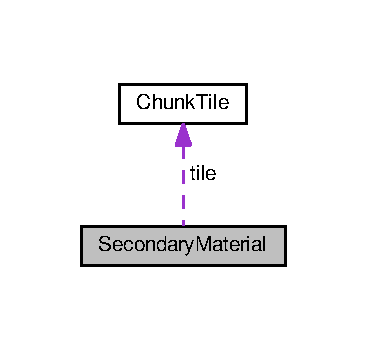
\includegraphics[width=176pt]{classSecondaryMaterial__coll__graph}
\end{center}
\end{figure}
\subsection*{Public Member Functions}
\begin{DoxyCompactItemize}
\item 
\hypertarget{classSecondaryMaterial_a69b96c4aacf0309d95e0ce9270ff74ad}{{\bfseries Secondary\-Material} (nlohmann\-::json)}\label{classSecondaryMaterial_a69b96c4aacf0309d95e0ce9270ff74ad}

\end{DoxyCompactItemize}
\subsection*{Public Attributes}
\begin{DoxyCompactItemize}
\item 
\hypertarget{classSecondaryMaterial_a2f6dbbe3c785234d802e193e20784307}{\hyperlink{classChunkTile}{Chunk\-Tile} {\bfseries tile}}\label{classSecondaryMaterial_a2f6dbbe3c785234d802e193e20784307}

\item 
\hypertarget{classSecondaryMaterial_a13a32cb245d947c7f7a5d7e904ace8b1}{float {\bfseries min\-Depth}}\label{classSecondaryMaterial_a13a32cb245d947c7f7a5d7e904ace8b1}

\item 
\hypertarget{classSecondaryMaterial_aac62f19526e18476aba6b7ebeba41cd6}{float {\bfseries max\-Depth}}\label{classSecondaryMaterial_aac62f19526e18476aba6b7ebeba41cd6}

\item 
\hypertarget{classSecondaryMaterial_aebfb0894af42a44a46010ff6f3b45d5c}{bool {\bfseries has\-Min\-Depth}}\label{classSecondaryMaterial_aebfb0894af42a44a46010ff6f3b45d5c}

\item 
\hypertarget{classSecondaryMaterial_a91408bbd26707e4bd3f7159158d48525}{bool {\bfseries has\-Max\-Depth}}\label{classSecondaryMaterial_a91408bbd26707e4bd3f7159158d48525}

\item 
\hypertarget{classSecondaryMaterial_acb0fb055763493d6a15b04fdf6b3285b}{bool {\bfseries is\-Ore}}\label{classSecondaryMaterial_acb0fb055763493d6a15b04fdf6b3285b}

\item 
\hypertarget{classSecondaryMaterial_a8efd21aa89ac3bead26261e5812054f9}{float {\bfseries noise\-Mul}}\label{classSecondaryMaterial_a8efd21aa89ac3bead26261e5812054f9}

\end{DoxyCompactItemize}
\subsection*{Static Public Attributes}
\begin{DoxyCompactItemize}
\item 
\hypertarget{classSecondaryMaterial_ad4c8f6f600a842aa530af1bed2913343}{static constexpr auto {\bfseries T\-A\-G} = \char`\"{}Secondary\-Material\char`\"{}}\label{classSecondaryMaterial_ad4c8f6f600a842aa530af1bed2913343}

\end{DoxyCompactItemize}


The documentation for this class was generated from the following files\-:\begin{DoxyCompactItemize}
\item 
/home/travis/build/\-Z\-S\-A\-Inf\-Project/\-Project\-No\-Name/src/world/chunk/Chunk\-Generator.\-h\item 
/home/travis/build/\-Z\-S\-A\-Inf\-Project/\-Project\-No\-Name/src/world/chunk/Chunk\-Generator.\-cpp\end{DoxyCompactItemize}

\hypertarget{classState}{\section{State Class Reference}
\label{classState}\index{State@{State}}
}


Inheritance diagram for State\-:
\subsection*{Public Member Functions}
\begin{DoxyCompactItemize}
\item 
\hypertarget{classState_af2121f8eb52144b7a789214f15e3601a}{virtual void {\bfseries update} (std\-::chrono\-::microseconds delta\-Time)=0}\label{classState_af2121f8eb52144b7a789214f15e3601a}

\item 
\hypertarget{classState_abea822ddf8d4a55439a0040eba979afb}{virtual void {\bfseries render} (sf\-::\-Render\-Window $\ast$render\-Window)=0}\label{classState_abea822ddf8d4a55439a0040eba979afb}

\item 
\hypertarget{classState_a1cdec36e9ffad91ba7af560770601017}{virtual void {\bfseries tick} ()=0}\label{classState_a1cdec36e9ffad91ba7af560770601017}

\item 
\hypertarget{classState_a8fba10b9995ce898339f3b0d39234788}{{\bfseries State} (\hyperlink{classState}{State} \&other)=delete}\label{classState_a8fba10b9995ce898339f3b0d39234788}

\item 
\hypertarget{classState_a7ac6cc4de6723746df3dfb183b8eb84f}{\hyperlink{classState}{State} \& {\bfseries operator=} (\hyperlink{classState}{State} \&other)=delete}\label{classState_a7ac6cc4de6723746df3dfb183b8eb84f}

\end{DoxyCompactItemize}


The documentation for this class was generated from the following file\-:\begin{DoxyCompactItemize}
\item 
src/state/State.\-h\end{DoxyCompactItemize}

\hypertarget{classTile}{\section{Tile Class Reference}
\label{classTile}\index{Tile@{Tile}}
}


Represents \hyperlink{classTile}{Tile} -\/ 1x1 game block.  




{\ttfamily \#include $<$Tile.\-h$>$}



Collaboration diagram for Tile\-:
\nopagebreak
\begin{figure}[H]
\begin{center}
\leavevmode
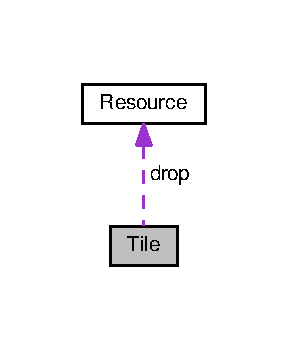
\includegraphics[width=154pt]{classTile__coll__graph}
\end{center}
\end{figure}
\subsection*{Public Member Functions}
\begin{DoxyCompactItemize}
\item 
\hypertarget{classTile_a135790fef385f3021dccf9dde464432c}{{\bfseries Tile} (nlohmann\-::json json)}\label{classTile_a135790fef385f3021dccf9dde464432c}

\item 
\hypertarget{classTile_a48792543e2c2b7b61b5ad2970f496b0e}{{\bfseries Tile} (std\-::string \hyperlink{classTile_aa5408d0f0f4a60f25796f651db2f84ac}{name}, float \hyperlink{classTile_accd68364f51cf745c5c95717a164b2e9}{hardness}, std\-::string \hyperlink{classTile_a4792f343c63f2b7c1bf1a7321ba60206}{terminal\-\_\-representation}, int \hyperlink{classTile_ac1b8010b027d438ee826af235dc00fe1}{texture\-\_\-x}, int \hyperlink{classTile_addde9f80a365eae65b1f4bc156f18722}{texture\-\_\-y}, bool \hyperlink{classTile_a3a32e61b42ec4bc8bb1d924261c19403}{is\-Solid}, int \hyperlink{classTile_ae2d870936fb8ae7df7fdd74f4cb27035}{category})}\label{classTile_a48792543e2c2b7b61b5ad2970f496b0e}

\end{DoxyCompactItemize}
\subsection*{Public Attributes}
\begin{DoxyCompactItemize}
\item 
\hypertarget{classTile_a4ed599912d54c30651137115ac15a91e}{\hyperlink{structResource}{Resource} {\bfseries build\-Cost}}\label{classTile_a4ed599912d54c30651137115ac15a91e}

\item 
\hypertarget{classTile_aeaeeec2011bc127120fdd3447d623235}{\hyperlink{structResource}{Resource} {\bfseries drop}}\label{classTile_aeaeeec2011bc127120fdd3447d623235}

\item 
\hypertarget{classTile_aa5408d0f0f4a60f25796f651db2f84ac}{std\-::string \hyperlink{classTile_aa5408d0f0f4a60f25796f651db2f84ac}{name}}\label{classTile_aa5408d0f0f4a60f25796f651db2f84ac}

\begin{DoxyCompactList}\small\item\em \hyperlink{classTile}{Tile} name showed to player. \end{DoxyCompactList}\item 
\hypertarget{classTile_accd68364f51cf745c5c95717a164b2e9}{float \hyperlink{classTile_accd68364f51cf745c5c95717a164b2e9}{hardness}}\label{classTile_accd68364f51cf745c5c95717a164b2e9}

\begin{DoxyCompactList}\small\item\em Hardness of a material. Correlates to time needed to destroy. \end{DoxyCompactList}\item 
\hypertarget{classTile_a4792f343c63f2b7c1bf1a7321ba60206}{std\-::string \hyperlink{classTile_a4792f343c63f2b7c1bf1a7321ba60206}{terminal\-\_\-representation}}\label{classTile_a4792f343c63f2b7c1bf1a7321ba60206}

\begin{DoxyCompactList}\small\item\em String used to represent tile in terminal for debug. \end{DoxyCompactList}\item 
\hypertarget{classTile_ac1b8010b027d438ee826af235dc00fe1}{int \hyperlink{classTile_ac1b8010b027d438ee826af235dc00fe1}{texture\-\_\-x}}\label{classTile_ac1b8010b027d438ee826af235dc00fe1}

\begin{DoxyCompactList}\small\item\em Integer x coordinate of texture on texture map. \end{DoxyCompactList}\item 
\hypertarget{classTile_addde9f80a365eae65b1f4bc156f18722}{int \hyperlink{classTile_addde9f80a365eae65b1f4bc156f18722}{texture\-\_\-y}}\label{classTile_addde9f80a365eae65b1f4bc156f18722}

\begin{DoxyCompactList}\small\item\em Integer y coordinate of texture on texture map. \end{DoxyCompactList}\item 
\hypertarget{classTile_a3a32e61b42ec4bc8bb1d924261c19403}{bool \hyperlink{classTile_a3a32e61b42ec4bc8bb1d924261c19403}{is\-Solid}}\label{classTile_a3a32e61b42ec4bc8bb1d924261c19403}

\begin{DoxyCompactList}\small\item\em Tells if entity can pass through. \end{DoxyCompactList}\item 
\hypertarget{classTile_ae2d870936fb8ae7df7fdd74f4cb27035}{int \hyperlink{classTile_ae2d870936fb8ae7df7fdd74f4cb27035}{category}}\label{classTile_ae2d870936fb8ae7df7fdd74f4cb27035}

\begin{DoxyCompactList}\small\item\em Category of the tile. \end{DoxyCompactList}\end{DoxyCompactItemize}
\subsection*{Static Public Attributes}
\begin{DoxyCompactItemize}
\item 
\hypertarget{classTile_a132be67261c6302553fa1114e4319c0c}{static constexpr auto {\bfseries T\-A\-G} = \char`\"{}Tile\char`\"{}}\label{classTile_a132be67261c6302553fa1114e4319c0c}

\end{DoxyCompactItemize}


\subsection{Detailed Description}
Represents \hyperlink{classTile}{Tile} -\/ 1x1 game block. 

\hyperlink{classTile}{Tile} can be created passing all fields (for debug) or using a J\-S\-O\-N object 

The documentation for this class was generated from the following files\-:\begin{DoxyCompactItemize}
\item 
/home/travis/build/\-Z\-S\-A\-Inf\-Project/\-Project\-No\-Name/src/tile/Tile.\-h\item 
/home/travis/build/\-Z\-S\-A\-Inf\-Project/\-Project\-No\-Name/src/tile/Tile.\-cpp\end{DoxyCompactItemize}

\hypertarget{classTileDatabase}{\section{Tile\-Database Class Reference}
\label{classTileDatabase}\index{Tile\-Database@{Tile\-Database}}
}


Singleton mapping ids to tiles.  




{\ttfamily \#include $<$Tile\-Database.\-h$>$}

\subsection*{Public Member Functions}
\begin{DoxyCompactItemize}
\item 
\hypertarget{classTileDatabase_a416e304c465d358759c5f75c2d9dd339}{{\bfseries Tile\-Database} (\hyperlink{classTileDatabase}{Tile\-Database} const \&)=delete}\label{classTileDatabase_a416e304c465d358759c5f75c2d9dd339}

\item 
\hypertarget{classTileDatabase_a6fea9bd536a262734b09a39e5b737250}{void {\bfseries operator=} (\hyperlink{classTileDatabase}{Tile\-Database} const \&)=delete}\label{classTileDatabase_a6fea9bd536a262734b09a39e5b737250}

\item 
void \hyperlink{classTileDatabase_a986e55f0705dbfb5428931563eff1497}{load\-Tiles} (std\-::string file)
\begin{DoxyCompactList}\small\item\em Loads tiles from J\-S\-O\-N file. \end{DoxyCompactList}\item 
\hypertarget{classTileDatabase_a1eb9f7c3ff7e497bada7a1475fb271f4}{void \hyperlink{classTileDatabase_a1eb9f7c3ff7e497bada7a1475fb271f4}{load\-Texture} (std\-::string file)}\label{classTileDatabase_a1eb9f7c3ff7e497bada7a1475fb271f4}

\begin{DoxyCompactList}\small\item\em Loads texture map for tiles from file. \end{DoxyCompactList}\item 
\hypertarget{classTileDatabase_afd8392440590a9a162104d27f93001a8}{\hyperlink{classTile}{Tile} \& {\bfseries operator\mbox{[}$\,$\mbox{]}} (int index)}\label{classTileDatabase_afd8392440590a9a162104d27f93001a8}

\end{DoxyCompactItemize}
\subsection*{Static Public Member Functions}
\begin{DoxyCompactItemize}
\item 
\hypertarget{classTileDatabase_a305f67578059fc81b04b0c99f3065e8d}{static \hyperlink{classTileDatabase}{Tile\-Database} \& {\bfseries get} ()}\label{classTileDatabase_a305f67578059fc81b04b0c99f3065e8d}

\end{DoxyCompactItemize}
\subsection*{Public Attributes}
\begin{DoxyCompactItemize}
\item 
\hypertarget{classTileDatabase_a3368141d1a148afb5830ff86b3ca29f6}{sf\-::\-Texture \hyperlink{classTileDatabase_a3368141d1a148afb5830ff86b3ca29f6}{texture}}\label{classTileDatabase_a3368141d1a148afb5830ff86b3ca29f6}

\begin{DoxyCompactList}\small\item\em Texture map for tiles. \end{DoxyCompactList}\end{DoxyCompactItemize}


\subsection{Detailed Description}
Singleton mapping ids to tiles. 

Contains vector of reference tiles. Loaded from json file using \hyperlink{classTileDatabase_a986e55f0705dbfb5428931563eff1497}{load\-Tiles()}. 

\subsection{Member Function Documentation}
\hypertarget{classTileDatabase_a986e55f0705dbfb5428931563eff1497}{\index{Tile\-Database@{Tile\-Database}!load\-Tiles@{load\-Tiles}}
\index{load\-Tiles@{load\-Tiles}!TileDatabase@{Tile\-Database}}
\subsubsection[{load\-Tiles}]{\setlength{\rightskip}{0pt plus 5cm}void Tile\-Database\-::load\-Tiles (
\begin{DoxyParamCaption}
\item[{std\-::string}]{file}
\end{DoxyParamCaption}
)}}\label{classTileDatabase_a986e55f0705dbfb5428931563eff1497}


Loads tiles from J\-S\-O\-N file. 

File should be a J\-S\-O\-N vector of tiles. 
\begin{DoxyParams}{Parameters}
{\em file} & -\/ path to file (root directory is res/) \\
\hline
\end{DoxyParams}


The documentation for this class was generated from the following files\-:\begin{DoxyCompactItemize}
\item 
/home/travis/build/\-Z\-S\-A\-Inf\-Project/\-Project\-No\-Name/src/tile/Tile\-Database.\-h\item 
/home/travis/build/\-Z\-S\-A\-Inf\-Project/\-Project\-No\-Name/src/tile/Tile\-Database.\-cpp\end{DoxyCompactItemize}

\hypertarget{classWorld}{\section{World Class Reference}
\label{classWorld}\index{World@{World}}
}
\subsection*{Public Member Functions}
\begin{DoxyCompactItemize}
\item 
\hypertarget{classWorld_ad41d823a21794ad47ac4478677b0ae7f}{void {\bfseries render} (sf\-::\-Render\-Window \&window, sf\-::\-View camera)}\label{classWorld_ad41d823a21794ad47ac4478677b0ae7f}

\item 
\hypertarget{classWorld_a6bba777d3b8230e5d84333b14ff9a559}{\hyperlink{structchunkTile}{chunk\-Tile} \hyperlink{classWorld_a6bba777d3b8230e5d84333b14ff9a559}{get\-Tile} (int x, int y)}\label{classWorld_a6bba777d3b8230e5d84333b14ff9a559}

\begin{DoxyCompactList}\small\item\em Gets \hyperlink{structchunkTile}{chunk\-Tile} using global coordinates of the world. \end{DoxyCompactList}\item 
\hypertarget{classWorld_a7d1aeeafb60622886696ac01d7cbef34}{void \hyperlink{classWorld_a7d1aeeafb60622886696ac01d7cbef34}{set\-Tile} (int x, int y, \hyperlink{structchunkTile}{chunk\-Tile} value)}\label{classWorld_a7d1aeeafb60622886696ac01d7cbef34}

\begin{DoxyCompactList}\small\item\em Sets tile to given value using global coordinates of the world. \end{DoxyCompactList}\item 
short \hyperlink{classWorld_a1bbfac1b517a991c30aa96b57d04d265}{mine\-Tile} (int x, int y)
\begin{DoxyCompactList}\small\item\em Mines given tile. \end{DoxyCompactList}\item 
\hypertarget{classWorld_a4598832293e050abba792d1b4367a368}{{\bfseries World} (int seed)}\label{classWorld_a4598832293e050abba792d1b4367a368}

\end{DoxyCompactItemize}
\subsection*{Static Public Attributes}
\begin{DoxyCompactItemize}
\item 
\hypertarget{classWorld_a9ebf0ccc9a330d5f3e4ed8401d64e5f6}{static constexpr auto {\bfseries T\-A\-G} = \char`\"{}World\char`\"{}}\label{classWorld_a9ebf0ccc9a330d5f3e4ed8401d64e5f6}

\end{DoxyCompactItemize}


\subsection{Member Function Documentation}
\hypertarget{classWorld_a1bbfac1b517a991c30aa96b57d04d265}{\index{World@{World}!mine\-Tile@{mine\-Tile}}
\index{mine\-Tile@{mine\-Tile}!World@{World}}
\subsubsection[{mine\-Tile}]{\setlength{\rightskip}{0pt plus 5cm}short World\-::mine\-Tile (
\begin{DoxyParamCaption}
\item[{int}]{x, }
\item[{int}]{y}
\end{DoxyParamCaption}
)}}\label{classWorld_a1bbfac1b517a991c30aa96b57d04d265}


Mines given tile. 

Mines tile at given coord 
\begin{DoxyParams}{Parameters}
{\em x} & X world coordinate \\
\hline
{\em y} & Y world coordinate \\
\hline
\end{DoxyParams}
\begin{DoxyReturn}{Returns}
tile id B\-E\-F\-O\-R\-E mining 
\end{DoxyReturn}


The documentation for this class was generated from the following files\-:\begin{DoxyCompactItemize}
\item 
src/world/World.\-h\item 
src/world/World.\-cpp\end{DoxyCompactItemize}

%--- End generated contents ---

% Index
\newpage
\phantomsection
\addcontentsline{toc}{chapter}{Index}
\printindex

\end{document}
